\documentclass{beamer}
%\documentclass[handout,t]{beamer}

\batchmode
% \usepackage{pgfpages}
% \pgfpagesuselayout{4 on 1}[letterpaper,landscape,border shrink=5mm]

\usepackage{amsmath,amssymb,enumerate,epsfig,bbm,calc,color,ifthen,capt-of,float}
\usepackage{algorithm2e}
\usepackage{algorithmic}
\usepackage{movie15}



\usetheme{Berlin}

\usecolortheme{mit}

\title{Hierarchical Leader Election Algorithm With Remoteness Constraint}
\author{Mohamed Tbarka}
\date{\today}
\pgfdeclareimage[height=0.5cm]{mit-logo}{ensias-logo.pdf}
\logo{\pgfuseimage{mit-logo}\hspace*{0.3cm}}

\AtBeginSection[]
{
  \begin{frame}<beamer>
    \frametitle{Outline}
    \tableofcontents[currentsection]
  \end{frame}
}
\beamerdefaultoverlayspecification{<+->}
% -----------------------------------------------------------------------------
\begin{document}
% -----------------------------------------------------------------------------

\frame{\titlepage}

\section[Outline]{}
\begin{frame}{Outline}

  \tableofcontents
\end{frame}

% -----------------------------------------------------------------------------
\section{Introduction}
\subsection{Leader Election Problem}
\begin{frame}{What is the problem of leader election ?}
Leader election is an important primitive for distributed computing, useful as a sub-routine for any application that requires the selection of a unique processor among multiple candidate processors (video conferencing, multi-player games, ...).
\end{frame}

\begin{frame}{What is distributed computing ?}
Distributed computing is a model in which components of a software system are shared among multiple computers to improve efficiency and performance.
\end{frame}

\subsection{State of art}
\begin{frame}{State of art}
	\begin{figure}
		\centering
		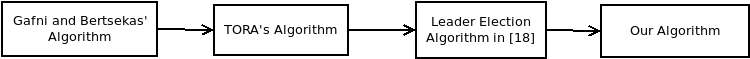
\includegraphics[width=1\linewidth]{../state_of_art}
		\caption{}
		\label{fig:stateofart}
	\end{figure}
\end{frame}
\iffalse
\begin{frame}{The Bully Algorithm}
  As a first example, consider the bully algorithm devised by Garcia-Molina (1982). When any process notices that the coordinator is no longer responding to requests, it initiates an election. A process, P, holds an election as follows:
  \pause
  \begin{itemize}
    \item <2-> $P$ sends an $ELECTION$ message to all processes with higher numbers.
    \item <3-> If no one responds, $P$ wins the election and becomes coordinator.
    \item <4-> If one of the higher-ups answers, it takes over. $P$'s job is done.
  \end{itemize}
\end{frame}

\begin{frame}
	\begin{figure}
		\centering
		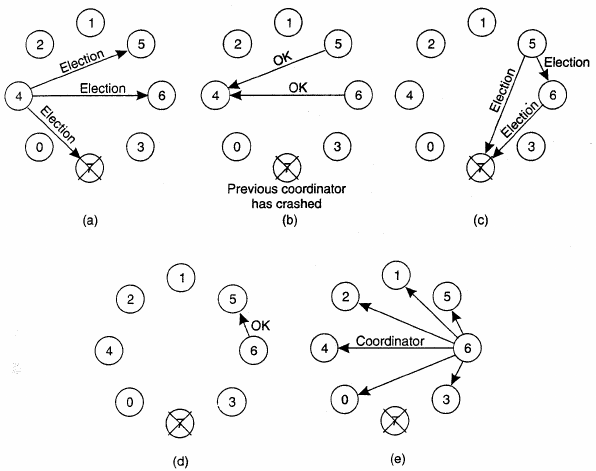
\includegraphics[width=0.7\linewidth]{bully_algorithm}
		\caption{Bully Algorithm}
		\label{fig:bullyalgorithm}
	\end{figure}
\end{frame}
\fi
% -----------------------------------------------------------------------------
\section{Preliminaries}
\subsection{System Model}

\begin{frame}{System Model}

\begin{itemize}
	\item The system is consisting of a set $P$ of computing nodes and a set $\chi$ of directed communication channels from one node to another node.
	\item The whole system as a set of (infinite) state machines that interact through shared events.

\end{itemize}

\end{frame}

\begin{frame}{System Model}

\begin{itemize}
	\item The system is consisting of a set $P$ of computing nodes and a set $\chi$ of directed communication channels from one node to another node.
	\item The whole system as a set of (infinite) state machines that interact through shared events.
	
\end{itemize}

\end{frame}
\begin{frame}{Asynchronous Dynamic Links' Model}

	The state of $Channel(u, v)$, which models the communication channel from node u to node v, consists of:
	\begin{itemize}
		\item a $status_{uv}$ variable;
		\item and a queue $mqueue_{uv}$ of messages.
	\end{itemize}
	 

\end{frame}

\begin{frame}{Configurations \& Executions}

\begin{itemize}
	\item The notion of configuration is used to capture an instantaneous snapshot of the state of the entire system.
	\item A configuration is a vector of node states, one for each node in $P$, and a vector of channel states, one for each channel in $\chi$.
\end{itemize}

\end{frame}

\begin{frame}{Configurations \& Executions}
In an initial configuration:
\begin{itemize}
	\item each node is in an initial state (according to its algorithm), \item for each channel $Channel(u, v)$, $mqueue_{uv}$ is empty, and \item for all nodes $u$ and $v$, $status_{uv} = status_{vu}$ (i.e., either both channels between $u$ and $v$ are up, or both are down).
\end{itemize}
\end{frame}

\begin{frame}{Configurations \& Executions}
	An execution is an infinite sequence $C_0, e_1 ,C_1, e_2, C_2 , ...$ of alternating configurations and events, starting with an initial configuration and, if finite, ending with a configuration.
\end{frame}


\subsection{Problem Definition}
\begin{frame}{Problem Definition}
Each node $u$ in the system has :
\begin{itemize}
	\item a local variable $lid_{u}$ to hold the $id$ of the supreme leader;
	\item another local variable $slid_u$ to hold the identifier of the sub-leader whose remoteness towards $u$ obeys the constraint.
\end{itemize}
\end{frame}

% -----------------------------------------------------------------------------
\section{H. Leader Election Algorithm}
\subsection{Informal Description}
\begin{frame}{Informal description}
After a leader is gone, the algorithm consists on three waves:
\begin{itemize}
	\item First wave : initiated by one of the lost leader's neighbors looking for it;
	\item Second wave : initiated by the node located at the edge of the network if the search has hit a dead-end;
	\item Third wave : initiated by the same node which initiated the first wave updating the other nodes' heights and constructing the spanning tree.
\end{itemize}

\end{frame}

\subsection{Nodes, Neighbors and Heights}

\begin{frame}{Nodes, Neighbors and Heights}
\begin{itemize}
	\item When a node $u$ gets a $ChannelUp$ event for the channel from $u$ to $v$, it puts $v$ in a local set variable called $forming_u$.
	\item When $u$ subsequently receives a message from $v$, it moves $v$ from its $forming_u$ set to a local set variable called $N_u$ ($N$ for neighbor).
	\item If $u$ gets a message from a node which is neither in its forming set, nor in $N_u$, it ignores that message.
	\item And when u gets a $ChannelDown$ event for the channel from $u$ to $v$, it removes $v$ from $forming_u$ or $N_u$ , as appropriate. 
\end{itemize}
   And when u gets a ChannelDown event for the channel from u to v, it
\end{frame}

\subsection{Initial State}
\begin{frame}{Initial State}
\begin{list}{--}
	\item $forming_u$ is empty,
	\item $N_u$ equals the set of neighbors of $u$ in $G^{init} _{chan}$
	\item $height_u[u] = (0, 0, 0, \delta _u , 0, l, u)$ where $l$ is the $id$ of a fixed node in $u's$ connected component in $G^{init} _{chan}$ (the current leader), and $\delta _u$ equals the distance from $u$ to $l$ in $G^{init} _{chan}$,
	\item for each $v$ in $N_u$, $height_u[v] = height_v[v]$ (i.e., $u$ has accurate information about $v$’s height), and
	\item $\mathcal{T} _u$ is initialized properly with respect to the definition of causal clocks.
\end{list}
\end{frame}


\subsection{Description Of The Algorithm}
\begin{frame}{Heights}

The height for each node is a 7-tuple of integers $((\tau , oid, r), \delta, (nlts, lid), id)$, where the first three components are referred to as the reference level ($RL$) and the fifth and sixth.

\begin{itemize}
	\item $\tau$, a non-negative timestamp which is either 0 or the value of the causal clock time when the current search for an alternate path to the leader was initiated.
	\item $oid$, is a non-negative value that is either 0 or the id of the node that started the current search (we assume node ids are positive integers).
	\item $r$, a bit that is set to 0 when the current search is initiated and set to 1 when the current search hits a dead end.
	\item $\delta$

\end{itemize}

\end{frame}


\subsection{Sample Execution}

\begin{frame}{The Code triggered by Update Message}
\begin{figure}[h]
	\centering
	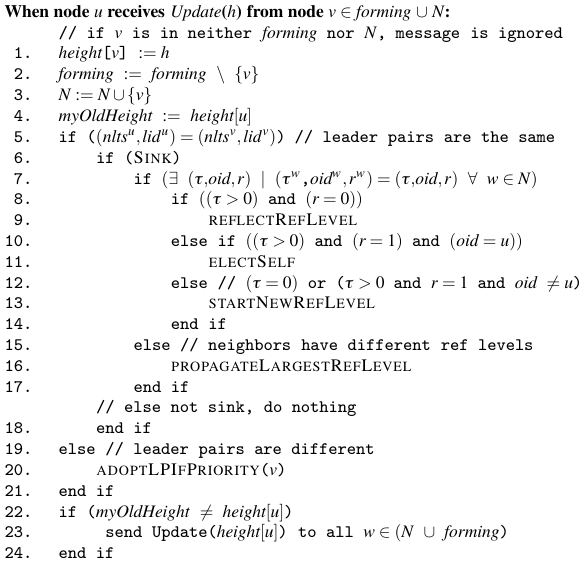
\includegraphics[width=0.5\linewidth]{tcode_update.png}
	%\caption{Code triggered by Update Message}
	\label{fig:figure1}
\end{figure}
\end{frame}

\begin{frame}{Subroutines}
\begin{figure}[h]
	\centering
	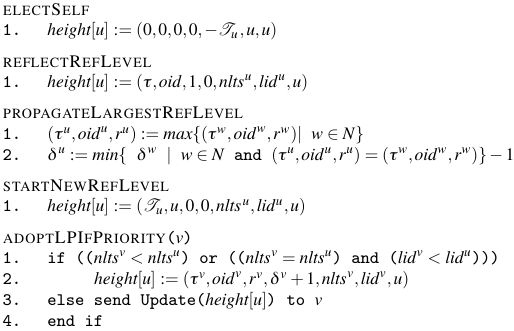
\includegraphics[width=0.8\linewidth]{subroutines.png}
	%\caption{Code triggered by Update Message}
	\label{fig:figure1}
\end{figure}
\end{frame}


% -----------------------------------------------------------------------------
\section{Correctness}

\subsection{Bounding the Number of Elections}

\subsection{Bounding the Number of New Reference Levels}

\subsection{Bounding the Number of Messages}
% -----------------------------------------------------------------------------

\section{Implementation}
\subsection{The Tool Used}

\begin{frame}{What's JBotSim ?}
JBoTSim is a java library that offers basic primitives for proto-typing, running, and visualizing distributed algorithms in dynamic networks.
\end{frame}

\subsection{Simulation}
\begin{frame}


\end{frame}

\subsection{Performance Test}
\begin{frame}{How is our algorithm's performance ?}
	\begin{figure}
		\centering
		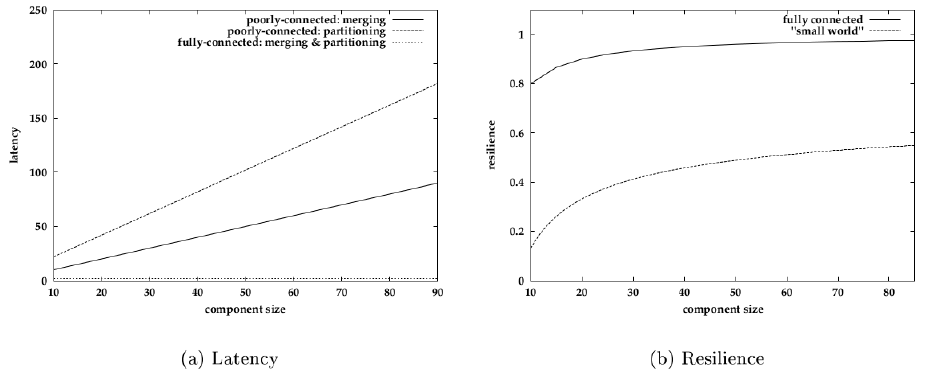
\includegraphics[width=1\linewidth]{performance_test}
		\caption{Simulation Results}
		\label{fig:performancetest}
	\end{figure}
	
\end{frame}

%----------------------------------------------------------------------------
\section{Conclusion}
\subsection{Is The Algorithm Perfect ?}
\begin{frame}{Is The Algorithm Perfect ?}
 An open question is how to extend our algorithm and its analysis to handle a wider range of clocks, such as approximately synchronized clocks and vector clocks.
\end{frame}

\begin{frame}{Question ?}
	
\end{frame}
% -----------------------------------------------------------------------------
\end{document}
